\documentclass[12pt]{article}

\usepackage{sbc-template}

\usepackage{graphicx,url}
\usepackage{color}
\usepackage{listings,comment}

%\usepackage[brazilian]{babel}   
\usepackage[utf8]{inputenc}


\lstdefinelanguage{NeoIDL}{
  sensitive = true, 
  keywords = {module, service, import, struct, path},
 %basicstyle=\normalfont\ttfamily,
    numbers=left,
    numberstyle=\scriptsize,
    stepnumber=1,
    numbersep=8pt,
    showstringspaces=false,
    breaklines=true,
    frame=lines,
    %backgroundcolor=\color{background}
}

\newcommand{\neoidl}{NeoIDL}
 

\sloppy

\title{Contratos REST robustos e leves:\\uma abordagem em Design-by-Contract
com NeoIDL}

\author{Lucas F. Lima\inst{1}\\Orientadores: Rodrigo Bonifácio de
Almeida\inst{2}, Edna Dias Canedo\inst{1}} 

\address{Departamento de Engenharia Elétrica -- Universidade de Brasília --
 UnB\\CEP 70910-900 -- Campus Darcy Ribeiro -- Asa Norte -- Brasília -- DF --
Brasil
\nextinstitute 
 Departamento de Ciência da Computação -- Universidade de Brasília -- UnB\\ CEP
 70910-900 -- Campus Darcy Ribeiro -- Asa Norte -- Brasília -- DF -- Brasil
\email{lucas.lima@aluno.unb.br, rbonifacio@cic.unb.br,
 ednacanedo@unb.br} 
}

\begin{document} 

\maketitle

\begin{center}

\center{Nível: Mestrado\\
Ano de Ingresso: 2014\\
Previsão de conclusão: Dezembro/2015\\
Aprovação da Proposta: Janeiro de 2014\\
Eventos Relacionados: SBES
}

\end{center}

\begin{resumo} 
  O trabalho de pesquisa de mestrado, sumarizado neste artigo, objetiva
  fortalecer a especificação de contratos para soluções concebidas sob o
  paradigma de computação orientada a serviços. A robustez é buscada por meio de
  construções que agregam \textit{Design-by-Contract} à linguagem \neoidl, de
  modo que os serviços especificados assegurem as pós-condições, desde que
  satisfeitas suas pré-condições.
  A proposta será submetida a validação empírica, verificando regras de
  transformações em um novo plugin para a \neoidl.
\end{resumo}

\newpage
\section{Introdução e Caracterização do Problema}\label{sec:introducao}

A computação orientada a serviços ( \emph{Service-oriented computing, SOC)} tem
se mostrado uma solução de \textit{design} de \textit{software} que favorece o
alinhamento às mudanças constantes e urgentes nas insituições
\cite{chen2008towards}. Os benefícios de SOC estão diretamente relacionados ao
baixo acoplamento dos serviços que compõem a solução, de forma que as partes
(nesse caso serviços) possam ser substituídas e evoluídas facilmente, ou ainda
rearranjadas em novas composições. Contudo, para que isso seja possível, é
necessário que os serviços possuam contratos bem definidos e independentes da
implementação.

Por outro lado, as linguagens de especificação de contratos para SOA apresentam
algumas limitações. Por exemplo, a linguagem WSDL (\emph{Web-services
description language}) \cite{zur2005developing} é considerada uma solução
verbosa que desestimula a abordagem \textit{Contract First}. Por essa razão,
especificações WSDL são usualmente derivadas a partir de anotações em código
fonte.
Além disso, os conceitos descritos em contratos na linguagem WSDL não são
diretamente mapeados aos elementos que compõem as interfaces do estilo
arquitetural REST (\emph{Representational State Transfer}).
Outras alternativas para REST, como Swagger e
RAML\footnote{http://raml.org/spec.html}, usam linguagens de propósito geral (em
particular JSON) adaptadas para especificação de contratos. Ainda que façam uso
de contratos mais sucintos que WSDL, essas linguagens não se
beneficiam da clareza típica das linguagens específicas para esse fim (como IDLs CORBA) e não oferecem
mecanismos semânticos de extensibilidade e modularidade.

Com o objetivo de mitigar esses problemas, a linguagem \neoidl foi proposta
para simplificar a especificação de serviços REST com mecanismos de modularização,
suporte a anotações, herança em tipos de dados definidos pelo desenvolvedor, e
uma sintaxe simples e concisa semelhante às \textit{Interface Description
Languages} -- IDLs -- presentes em \textit{Apache Thrift}\texttrademark e
CORBA\texttrademark. Por outro lado, a \neoidl, da mesma forma que WSDL, Swagger
e RAML não oferece construções para especificação de contratos formais de
comportamento como os presentes em linguagens que suportam DBC (\emph{Design by
Contract})~\cite{meyer1992applying}, como JML, Spec\# e Eiffel.

Dessa forma, os objetivos dessa pesquisa envolvem inicialmente investigar o uso
de construções DBC no contexto da computação orientada a serviços e conduzir uma
revisão sistemática da literatura para identificar os principais trabalhos que
lidam com a relação entre DBC e SOC. Em seguida especificar e implementar novas
construções para a linguagem \neoidl, de tal forma que seja possível especificar
contratos mais precisos; além de definir regras de transformação das novas
construções \neoidl para diferentes tecnologias (como Twisted) que suportam a
implementação de serviços em REST.
Por fim, conduzir uma validação empírica da proposta usando uma abordagem mais
exploratória, possivelmente usando a estratégia \emph{pesquisa-ação}.




\section{Fundamentação Teórica}\label{sec:fundamentacao}

SOC é um estilo arquitetural cujo objetivo é prover baixo acoplamento por meio
da interação entre agentes de software, chamados de serviços
\cite{he2003service}. A chave para que a solução baseada em SOC tenha
custo-benefício favorável é o reuso, o qual somente é possível se os serviços
possuírem interfaces ubíquas, com semânticas genéricas e disponíveis para seus
consumidores. Usualmente, a comunicação com os serviços, e entre eles, é feita
por meio da troca de mensagens com uso de \textit{servi\c cos web}, que seguem
padrões abertos de comunicação e que atuam sobre o protocolo HTTP. SOAP e
REST~\cite{fielding2000fielding} s\~{a}o as tecnologias mais usadas para
implementa\c c\~{a}o de servi\c cos web, sendo que REST tem atra\'{i}do um maior
interesse nos \'{u}ltimos anos.

Entre os oito princípios para desenvolvimento SOA descritos
em~\cite{erl2008soa}, existe um especial interesse no \emph{contrato
padronizado} (\textit{Standardized Service Contract}), que sugere que serviços
de um mesmo inventário devem seguir os mesmos padrões de \textit{design}, de
modo a favorecer o reuso e composição. Este princípio prega a abordagem
\textit{Contract First}, em que a concepção do serviço parte da especificação do
contrato e não com a geração do contrato a partir código. \'{E} importante
destacar que n\~{a}o existe um padr\~{a}o para especificar contratos em REST, o
que motivou o desenho da \neoidl~\cite{bonifacio2015neoidl}, uma linguagem
espec\'{i}fica do dom\'{i}nio para especificação de contratos REST e que,
diferente das linguagens existents, prov\^{e} recursos de modularidade e herança
de tipos de dados customizados. Utilizando uma abordagem transformacional, a
\neoidl{} oferece suporte ferramental que gera c\'{o}digo fonte para diferentes
linguagens e plataformas REST, a partir de um conjunto de módulos \neoidl{} onde
são especificados os tipos de dados e os serviços.

A Figura \ref{lst:modulobasiconeo} apresenta um exemplo de módulo \neoidl{}
com a defini\c c\~{a}o de um tipo de dados \texttt{ItemDoCatalogo} e duas
opera\c c\~{o}es (chamadas de capacidades na terminologia REST):
\texttt{atualizarItem} (opera\c c\~{a}o do tipo POST associada ao
\emph{endpoint} \texttt{catalogo}) e \texttt{pesquisarItem} (opera\c c\~{a}o do
tipo GET, do mesmo \emph{endpoint}).


\begin{figure}[htb]
\begin{scriptsize}
\lstinputlisting[language=NeoIDL,firstnumber=1]{getCharactersDbc.tex}
\end{scriptsize}
\caption{Exemplo de um módulo escrito em \neoidl}
\label{lst:modulobasiconeo}
\end{figure}


Conforme mencionado, o suporte ferramental da \neoidl{} processa um conjunto de
módulos escritos na linguagem \neoidl{}, gerando o código com a estrutura para
implementação dos serviços descritos.
A versão atual do ambiente \neoidl{} suporta geração de códigos em Java e Python
para as plataformas \emph{neoCortex}\footnote{propriet\'{a}ria do Ex\'{e}rcito
Brasileiro} e \emph{Twisted}. Entretanto, esse ambiente é extensível por meio
da implementação de novos plugins~\cite{bonifacio2015neoidl}.


%% \begin{figure}[ht] \centering
%% 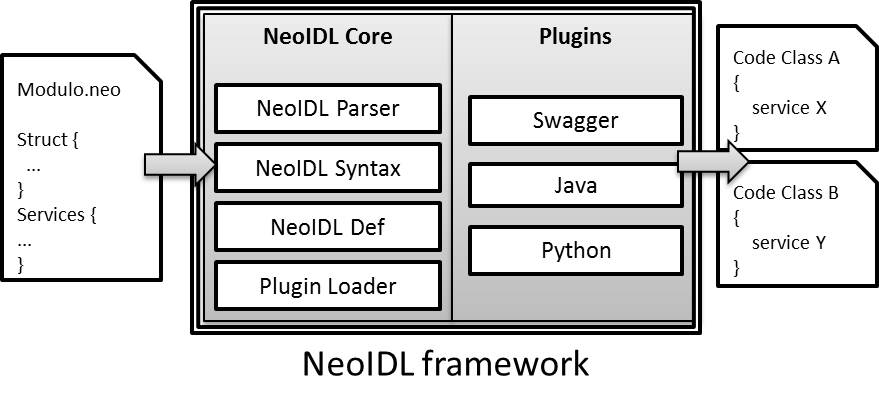
\includegraphics[width=.5\textwidth]{NeoIDLFrameworkArchtecture.jpg}
%% \caption{Entradas (lado esquerdo) e saídas (lado direito) do \textit{framework}
%% \neoidl}
%% \label{fig:NeoFrameArch}
%% \end{figure}

\emph{Limita\c c\~{a}o da \neoidl}. Atualmente a \neoidl{} permite apenas a
especifica\c c\~{a}o de \emph{weak contracts}, o que n\~{a}o permite estabelecer
obriga\c c\~{o}es entre fornecedores e clientes de servi\c cos. Esse tipo de
obriga\c c\~{a}o pode ser estabelecida com alguma t\'{e}cnica de
\emph{Design-by-contract}~\cite{meyer1992applying} (DBC) -- na qual o consumidor
e o fornecedor de servi\c cos firmam entre si um conjunto de garantias. Em um
contexto mais simples, de um lado o consumidor deve garantir que, antes da
chamada a um servi\c co (ou um m\'{e}todo de uma classe), os parâmetros de
entrada devem ser respeitados (essas garantias s\~{a}o denominadas de
pré-condições). Do outro lado, o fornecedor deve garantir que, uma vez
respeitadas as pré-condições, as propriedades relacionadas ao sucesso da
execução (pós-condições) s\~{a}o preservadas. DBC tem o objetivo de aumentar a
robustez do sistema e tem na linguagem Eiffel \cite{meyer1991eiffel} um de seus
precursores. O uso de DBC na concepção de sistemas, segundo
\cite{EiffelDBC:2012} é uma abordagem sistemática que tende a reduzir a
quantidade de erros observados nos sistemas.
Mais recentemente, algumas t\'{e}cnicas de \emph{design-by-contract} foram
especificadas e implementadas para outras linguagens de programa\c c\~{a}o, como
JML para a linguagem Java~\cite{leavens} e \texttt{Spec\#} para a linguagem
\texttt{C\#} (e demais linguagens da plataforma .NET)~\cite{barthe}.

% \subsection{NeoIDL}


\section{Estado Atual do Trabalho}\label{sec:estadoAtual}

As constru\c c\~{o}es para especificar pré-condições e pós-condições\footnote{Não se identificou, até o
estágio atual da pesquisa, aplicabilidade de invariantes em
serviços REST.} na linguagem da NeoIDL est\~{a}o sendo definidas, de forma a
agregar às especifica\c c\~{o}es mecanismos para estabelecer as condições de execução e as garantias dos serviços. Note que, além da validação dos parâmetros de entrada e valores de retorno típicos do DBC, a abordagem proposta nessa disserta\c c\~{a}o permitirá a inclusão de chamadas a serviços REST como pré e pós condições. 
Para ilustrar algumas decis\~{o}es de projeto, a seguir s\~{a}o apresentados 
dois exemplos do uso da abordagem que est\'{a} sendo proposta. 

O trecho de módulo \neoidl{} constante da Figura~\ref{lst:DBCSimple} destaca a
capacidade \texttt{incluirItem} (l. 7). Para que se tenha o item incluído no
catálogo, é necessário fornecer um valor para o atributo descrição
(obrigatório). A pré-condição (l. 5) se inicia com a notação
\texttt{/@require} e possui validação sobre o atributo descrição. Note que o
atributo é precedido da palavra \texttt{old}, que indica o valor do atributo antes do processamento do
serviço. De forma an\'{a}loga, est\'{a} previsto o prefixo \texttt{new}, que
indica o valor do atributo após a execução do serviço. Na
Figura~\ref{lst:DBCSimple} ainda \'{e} estabelecida uma cláusula
\texttt{/@otherwise} (l. 6), estabelecendo que a falha no atendimento da
pré-condição deve levar a uma resposta com o código HTTP 412 (falha de
pré-condição).

\begin{figure}[htb]
\begin{scriptsize}
\lstinputlisting[language=NeoIDL,firstnumber=1]{DBCsimple.neo}
\end{scriptsize}
\caption{Exemplo da notação DBC na linguagem \neoidl}
\label{lst:DBCSimple}
\end{figure}

A Figura~\ref{lst:DBCService} apresenta a capacidade \texttt{excluirItem} (l.
8). Nesse caso são estabelecidas pré e pós condições, ambas com chamadas ao
serviço \texttt{Catalogo.pesquisarItem}. Antes da execução da capacidade
\texttt{excluirItem}, é verificado se o item exite. Caso exista, a pré-condição é
satisfeita e o item é excluído. A pós-condição (l. 6) confirma que o item não
consta mais do catálogo. Se a pré-condição não for satisfeita, a cláusula
\texttt{/@otherwise} (l. 7) informa ao cliente do serviço que o item não foi
localizado (código HTTP 404 - Objeto não encontrado).


\begin{figure}[htb]
\begin{scriptsize}
\lstinputlisting[language=NeoIDL,firstnumber=1]{DBCservice.neo}
\end{scriptsize}
\caption{Exemplo da notação DBC na linguagem \neoidl{} com chamada a serviço}
\label{lst:DBCService}
\end{figure}

Ou seja, a proposta envolve elementos concebidos na linguagem JML~\cite{leavens} 
(como as constru\c c\~{o}es \texttt{old} e \texttt{new}) com elementos 
t\'{i}picos do estilo arquitetural REST (chamadas 
a servi\c cos sem estado utilizando m\'{e}todos HTTP, sem\^{a}ntica de retorno 
das opera\c c\~{o}es observando os c\'{o}digos de retorno HTTP, etc.), os quais 
habilitam n\~{a}o apenas o estabelecimento de contratos mas tamb\'{e}m uma 
forma de guiar a composi\c c\~{a}o de servi\c cos. 
Novos \textit{plugins} \neoidl{} devem ser implementados para permitir chamadas
a serviços a partir de pré e pós condições. 

%% --- uma vez que a transforma\c c\~{a}o de c\'{o}digo 
%% com chamadas a servi\c c\os ainda não é possível com os plugins existentes. 
%% Conforme mencionado, a ideia é que essas chamadas se assemelhem a composição de serviços.

%% Há de se considerar, contudo, que está consolidado na indústria a implementação
%% de composição de serviços com o produto \textit{Enterprise Service Bus} -- ESB
%% \cite{schmidt2005enterprise}. Entretanto, o uso de ESB para
%% \textit{microservices} não é conveniente, em razão da granularidade dos
%% serviços.


%% Um novo plugin, com suporte a DBC, está sendo implementado no \neoidl
%% \textit{framework}. Uma vez que todos os serviços gerados seguirão o paradigma
%% REST, adotamos a tecnologia \textit{Python Twisted}, projetada para tratar os
%% protocolos de rede e flexível para permitir manipulação dos códigos
%% padrão HTTP (Forbiden, Not Found, Ok, etc), informando, assim, sucesso ou
%% insucesso nas pré e pós-condições.


%% Em termos de estudo de caso, o presente trabalho aborda o cenário de catálogo de
%% serviços. O uso de DBC será utilizado para verificação das controle de acesso na
%% inclusão e alterações de itens no catálogo.


\emph{Valida\c c\~{a}o.} Em paralelo \`{a} especifica\c c\~{a}o 
das extens\~{o}es de linguagem \neoidl{} e implementa\c c\~{a}o de 
plugins, est\'{a} sendo feito o planejamento da 
valida\c c\~{a}o da proposta -- que deve seguir uma abordagem 
de pesquisa-a\c c\~{a}o considerando cen\'{a}rios reais (possivelmente 
com exemplos do Ex\'{e}rcito Brasileiro, parceiro na 
concep\c c\~{a}o da primeira vers\~{a}o da \neoidl). Um cenário candidato é
de verificação de controle de acesso aos serviços, a partir de pré-condições com
chamada ao serviço de autorização, aplicando-se assim solução a um problema
real (pesquisa-a\c c\~{a}o). Serão empregadas técnicas de avaliação
empírica em engenharia de software \cite{shull2008guide} para coleta e
análise dos dados.

\section{Trabalhos Relacionados}\label{sec:trabRelacionados}

Verifica-se que, embora definido já há alguns anos, DBC continua
sendo objeto de pesquisa \cite{poyias2014design}, \cite{rubio2013verifying},
\cite{belhaouari2012design}. Nesse dois últimos casos, o estudo de caso está
associado a controle de acesso, cenários aderentes a que se pretende
atingir com esta pesquisa.

Durante a pesquisa bibliográfica, muito embora o primeiro princípio SOA
es\-ta\-be\-le\-ci\-do por \cite{erl2008soa} recomende \textit{Contract First},
não se identificou publicação que associasse diretamente \textit{Design-by-Contract} à
especificação de contratos SOA.

Os trabalhos que mais se aproximam são os de \cite{ling2003describing} e
\cite{heckel2005towards}. O primeiro define uma forma de \textit{Design-by-Contract} para
arquiteturas de \textit{workflow}. O autor considera, porém, que para grandes
arquiteturas, a complexidade aumenta o risco de falha de \textit{design}. Já
\cite{heckel2005towards} foca na especificação de modelos para DbC em Web
Services, não tratando a especificação concreta do contrato. Além disso, se
restringe a Web Services SOAP.



\renewcommand\refname{Referências}
\bibliographystyle{sbc}
\bibliography{sbc-template}

\end{document}
